\subsection{Kamov}
\begin{wrapfigure}{r}{0.5\textwidth}
  \begin{center}
    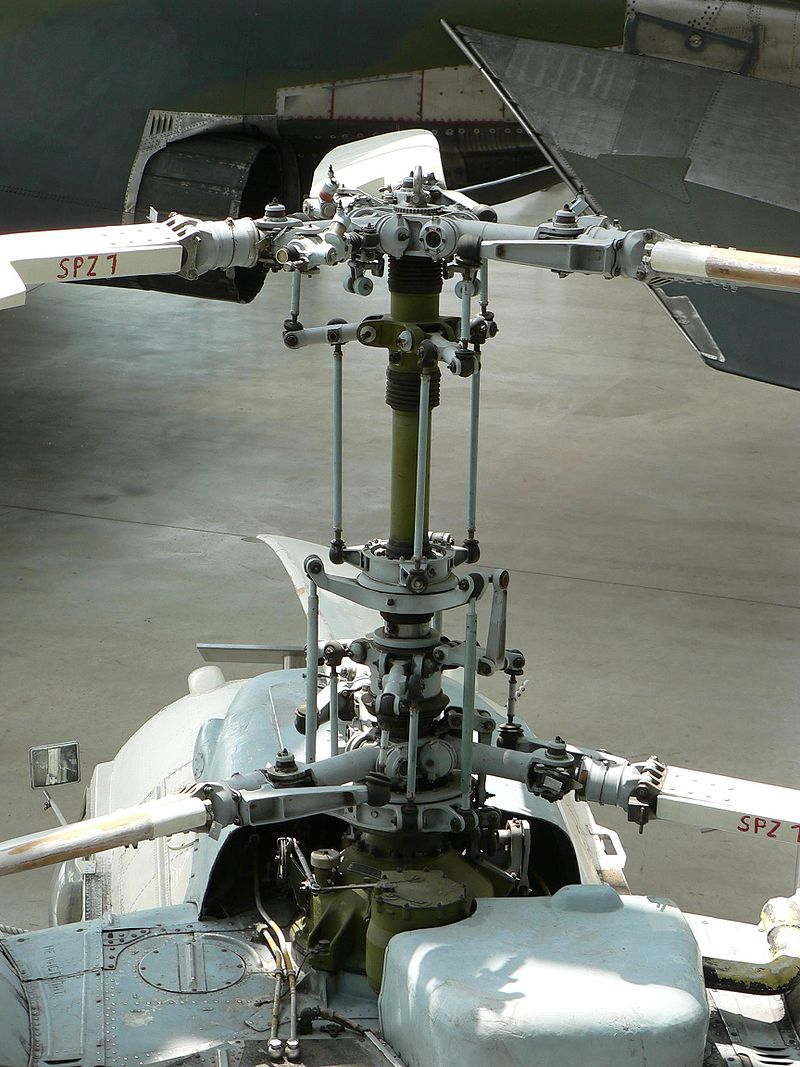
\includegraphics[width=0.28\textwidth]{images/kamov.jpg}
  \end{center}
  \caption{Ejemplo de imagen a la derecha no flotante}
\end{wrapfigure}
Kamov (en ruso: Камов) es un fabricante ruso de helicópteros, que ha heredado la fabricación de la antigua OKB-938 (en ruso: Особое Конструкторское Бюро), fundada en la Unión Soviética por Nikolái Kámov en el año 1948.


Kamov es una empresa especializada en la fabricación de helicópteros, que tienen como característica principal la de montar rotores coaxiales contrarrotativos.


En el año 2006 Mil se fusionó con Kamov y Rostvertol para formar la Corp. Oboronprom, la marca Kamov se mantendrá, pero se limitarán las nuevas líneas de productos.


Los rotores coaxiales cuentan con ciertas ventajas, entre ellas alta maniobrabilidad, fácil manejo y pequeñas dimensiones. Los helicópteros coaxiales son los de primer lugar en producción dentro del país y en el mundo, y se han convertido en el tipo de uso múltiple a bordo de helicópteros, caso del modelo Ka-15 (1957). Kamov es prácticamente la única empresa en el mundo que ha dominado los helicópteros con el esquema coaxial y a su vez ha implantado su producción a gran escala con aplicaciones prácticas, lo cual le ha permitido competir con éxito en el mercado frente a las principales compañías mundiales de helicópteros. 
